\documentclass[11pt,letterpaper]{article}

% --- Packages ---
\usepackage[margin=1in]{geometry}
\usepackage{amsmath,amssymb}
\usepackage{booktabs}
\usepackage{microtype}
\usepackage{xcolor}
\usepackage{titlesec}
\usepackage{hyperref}
\usepackage{graphicx}

\hypersetup{
    colorlinks=true,
    linkcolor=black,
    citecolor=blue!70!black,
    urlcolor=blue!70!black
}

\titleformat{\section}{\large\bfseries}{\thesection}{1em}{}[\titlerule]
\titleformat{\subsection}{\normalsize\bfseries}{\thesubsection}{1em}{}
\setlength{\parskip}{0.75em}
\setlength{\parindent}{0pt}

\title{\Large\textbf{UCI F1TENTH Autonomous Racing Stack Technical Specification}}
\author{\textbf{Jeffery Lee} \\ University of California, Irvine \\ F1TENTH at UCI}
\date{September 2026}    


\begin{document}

\maketitle

\section{Introduction}
The RoboRacer (previously F1TENTH) network is a collaborative effort founded at the University of Pennsylvania and led by professor Rahul Mangharam. 
The goal of RoboRacer is to provide a platform for competitions and research in the field of autonomous racing. 
The UCI F1TENTH team is a part of this network and has developed our own autonomous racing stack for 1/10th scale racing. 
In this document, we will provide an overview and guide to our system architecture and software stack, comprising the following: the vehicle, SLAM, and \textit{WarpoRacer}.

In a general scope, the race stack is an end-to-end autonomous navigation platform implemented in ROS 2. The sensor setup currently consists of a 2D Lidar and IMU odometry with future plans to integrate a depth camera.
The vehicle carries an NVIDIA Jetson Orin Nano as its computing unit and a VESC Controller for motor controls.
Our Simultaneous Localization and Mapping (SLAM) is done by Google Cartographer (under folder \texttt{roboracer\_slam}). 
For our autonomous racing approches, we developed \textit{WarpoRacer}, a highly efficient rigid-body simulator written with NVIDIA Warp for hardware acceleration.
\textit{WarpoRacer} allows us to perform rapid iterations of reinforcement learning updates and PPO policy training in the setting of a competition.

\vspace{1em}

\section{Vehicle Hardware and Sensors}
Operating 1/10th scale autonomous vehicles at speeds up to 18\,\text{m/s} requires a reliable chassis. For our purpose, a well-tuned chassis is critical to preserve sensor accuracy.
Minimizing the dynamic effects of aggressive turning and acceleration prevents tilting of the LiDAR and other sensors, ensuring consistent readings, as a fault could completely jeopardize the navigation systems.

\begin{table}[h]
\centering
\small
\caption{Summary of Core Compute and Perception Hardware}
\begin{tabular}{@{}lll@{}}
\toprule
\textbf{Category} & \textbf{Device} & \textbf{Primary Function} \\ \midrule
Compute Unit      & NVIDIA Jetson Orin Nano (500\,GB NVMe) & ROS 2, SLAM, and PPO policy \\
LiDAR             & Hokuyo UST-10LX Rangefinder            & 2D rangefinder for object avoidance \\
IMU               & 9-Axis IMU                             & Acceleration and rotation \\
Vision            & Intel RealSense D435i                  & Depth camera for 3D perception \\
\bottomrule
\end{tabular}
\end{table}

\subsection{Hardware Architecture}
\begin{figure}[h]
    \centering
    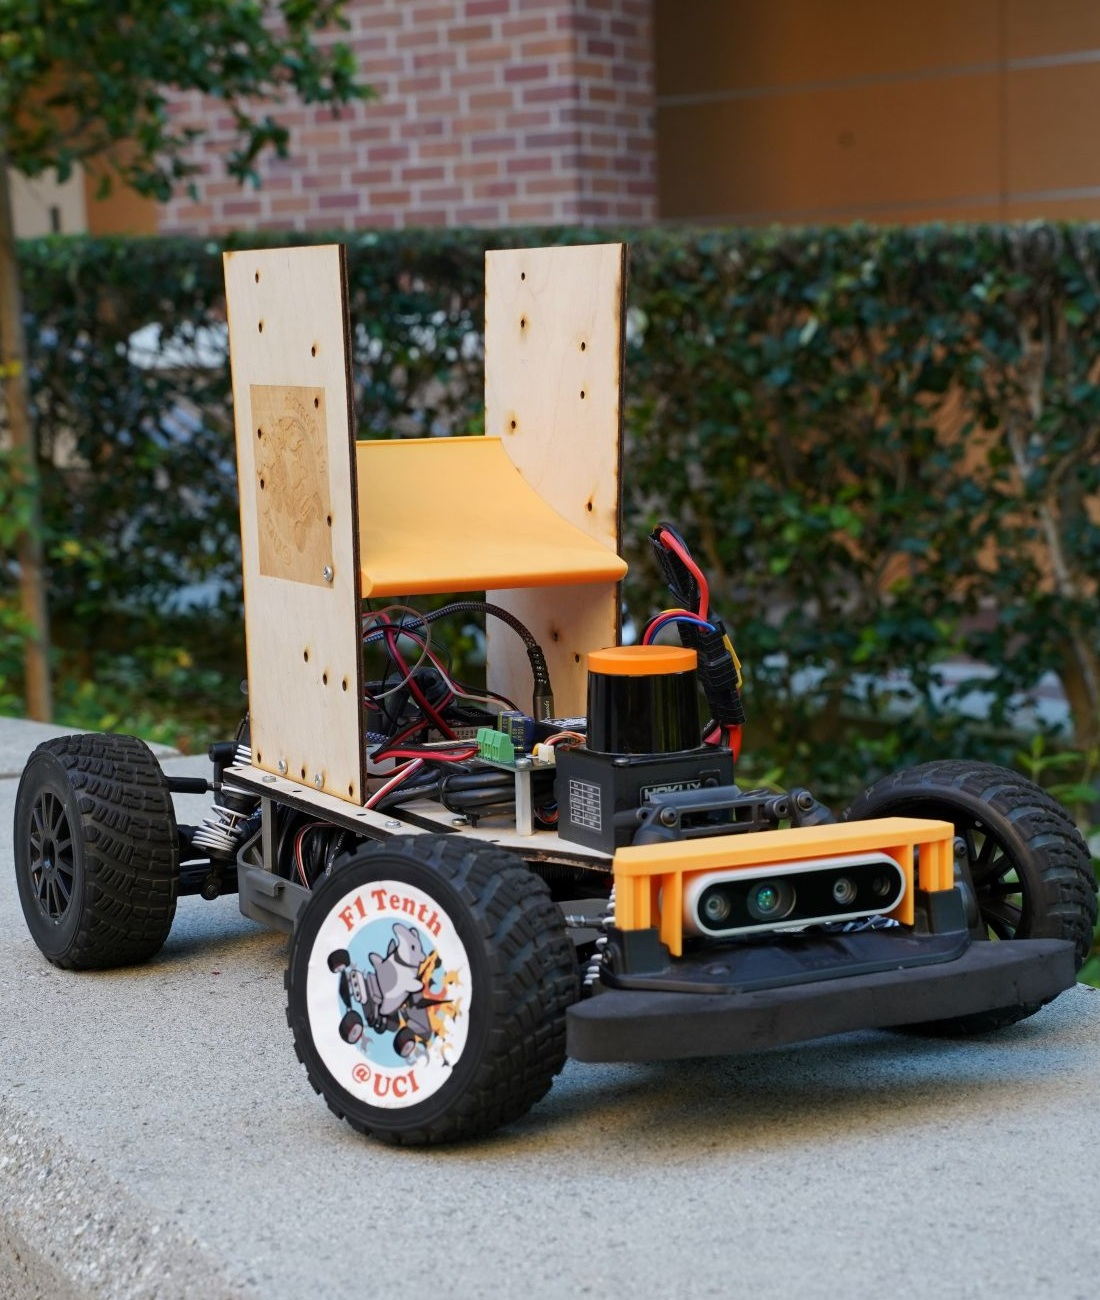
\includegraphics[width=0.7\textwidth]{car_hero}
    \caption{The UCI F1TENTH vehicle}
    \label{fig:F1TENTH}
\end{figure}

\begin{itemize}
    \item \textbf{Compute Module:} The NVIDIA Jetson Orin Nano runs Linux, and is responsible for every computation task that the vehicle performs.
    \item \textbf{Chassis:} The build is based on the 4-wheel drive Traxxas Fiesta ST Rally VXL Edition, with custom parts to allow for mounting of hardware.
    \item \textbf{Tires and Suspension:} The vehicle has an array of tires for varying surface conditions, and a suspension system that allows for spacing adjustments.
    \item \textbf{Motor Control:} We use the VESC 6 MkV TRAMPA controller to control the motor, powered by a 14.8\,\text{V} (65.1\,\text{Wh}) LiPo Battery. This also supports our IMU inputs.
    \item \textbf{Sensors:} The primary sensor is a Hokuyo UST-10LX LiDAR scanning a $270^\circ$ by $10\,\text{m}$ rated range (30\,\text{m} naxunyn) at 40\,\text{Hz}. The mount in the front of the vehicle also carries an Intel RealSense D435i depth camera.
\end{itemize}

\section{System Architecture and Repository Structure}
The complete software \href{https://github.com/uci-f1tenth/race_stack}{\texttt{race\_stack}} repository is containerized by Docker for ease of deployment and reproducibility on various OS platforms and cloud servers.
Our standard package installer is \href{https://docs.astral.sh/uv/}{\texttt{astral-uv}} for the same purpose. For additional information on how to set up the repository, refer to the \texttt{README.md} file.

The software section of the document will follow the chronological order in accordance with running the race stack.

\subsection{Simultaneous Localization and Mapping}
The SLAM algorithm is currently deployed primarily for generating maps of the race track used for training the PPO policy, since the PPO only requires direct observations to navigate. 
Localization will be integrated into the pipeline as we explore other methods in future iterations.

\begin{itemize}
    \item \textbf{\texttt{/roboracer\_slam}:} Google Cartographer is used for SLAM, and the ROS 2 node is located in this folder. The ROS node subscribes to the LiDAR and IMU topics, and publishes a map of the environment. The map is generated with loop closures, and is saved to a file for later use.
    \item \textbf{\texttt{/warpSLAM}:} A custom SLAM implementation that utilizes NVIDIA Warp for GPU acceleration. This implementation is still under development.
\end{itemize}

\subsection{Reinforcement Learning}
Reinforcement learning methods, such as Proximal Policy Optimization (PPO), require up to hundreds of millions of steps to converge. Standard Gym wrappers fall short in terms of efficiency, as they often render unnecessary graphics and perform physics calculations on the CPU.
As a solution, we developed \textit{WarpoRacer}, a GPU-accelerated rigid-body simulator that allows for parallelized simulation of multiple vehicles and race maps.

\begin{itemize}
    \item \textbf{\texttt{/warporacer}:} Our core simulation engine. It is capable of executing simple rigid-body physics and collisions across parallel instances simultaneously 
    within GPU CUDA kernels. NVIDIA Warp also helps accelerate the computation of 2D LiDAR rays, which are passed into PyTorch networks for PPO policy training.
    \item \textbf{Observation Space:} The observation is a 110 element array that consists of 108 downsampled LiDAR ray casts spanning a $270^\circ$ field of view along with the vehicle's current steering angle and its forward velocity.
    Since the PPO policy only sees readings from sensors with no map relevant data, the method requires no localization at run time, resulting in our choice to use SLAM primarily for map generation.
    \item \textbf{Action Space:} There are two values that the PPO policy will output. One being the steering rate and the other being acceleration.
    \item \textbf{Reward Function:} The policy is rewarded for progressing along the track centerline (calculated by the simulator) with a weight dependent on forward velocity. The policy receives
    penalties for track wall proximity and deviations off the centerline. Additionally, there is a set penalty for a collision, which will also end the training episode.
    \item \textbf{Visualization:} The simulator is capable of outputting 2D video visualizations of the vehicle's trajectory and other statistics such as episode return. These data can be found in Weights and Biases if the option was selected when running the training script.
\end{itemize}

\subsection{Physical Vehicle Deployment}
\begin{itemize}
    \item \textbf{\texttt{/warporacer\_node}:} A ROS 2 node that runs the trained PPO policy on the physical vehicle. It subscribes to the \texttt{/scan} and the \texttt{/odom} topics, and publishes drive commands to \texttt{/drive}. 
    The observations are constructed exactly as in training, so that the policy will see matching inputs in simulation and on the physical car.
    \item \textbf{Launching:} Refer to the \texttt{README.md} file for specific commands on launching the respective ROS 2 nodes for the desired task.
\end{itemize}

\subsection{Safety Constraints and Sanity Checks}
Because there are many confounding factors that can cause unexpected behavior on the physical vehicle, we have implemented various safety checks.
\begin{itemize}
    \item \textbf{\texttt{low\_voltage\_shutdown.py}:} A process that shuts the Jetson Orin Nano down if the LiPo battery voltage drops below 12\,\text{V}.
    \item \textbf{\texttt{calibrate.py}:} Simply sends the vehicle forward for 1\,\text{m} according to the VESC controller's odometry data. This is measured physically to check the VESC's speed and odometry tuning. Steering is not tuned through this script.
    \item \textbf{Deadman Switch:} A standalone script that does not exist in the repository. It is used to ensure that the vehicle will only run when the operator is actively holding down a button on a controller.
\end{itemize}

Additionally, we are able to tune some parameters through environment variables without having to rebuild the container. These can be found in the \texttt{README.md} file as well.

\subsection{Simulation Bridge}
Since we are using a custom Gym environment, we need a port to the official simulator \href{https://autodrive-ecosystem.github.io/}{AutoDrive}. The \texttt{f1tenth\_to\_autodrive\_bridge.py} script translates between the two
ROS 2 nodes.

\subsection{Classical Navigation Stacks}
This repository also includes two other classical approaches to navigation, which are not our main research focus, but are still useful for testing purposes.
\begin{itemize}
    \item \textbf{\texttt{/disparity\_extender}:} A LiDAR based reactive approach. It slides a fixed window of LiDAR scans and steers towards the window with the largest disparity (farthest distance to the obstacle).
    \item \textbf{\texttt{/pure\_pursuit}:} A controller that follows some closed race line on the track. This approach requires localization and is therefore implemented but awaiting localization integration.
\end{itemize}

\section{Conclusion and Future Outlook}
This documentation presented the mechanical and software foundations of the UCI F1TENTH autonomous race stack. Through our combination of approaches, 
we are able to iterate a new version of the PPO policy in under 10 minutes. In the past, this has given us significant operational advantages when the policy fails unexpectedly.
In the future, it is necessary to upgrade our simulator from 2D to 3D along with other improvements. This is due to the fact that competitions are evolving to include ramps, which \textit{WarpoRacer} 
will not be able to sufficiently handle. This will hopefully also improve our physics simulations, as it gives us a chance to be much more precise in our calculations to include parameters
such as pitch, roll, vertical load, etc.
\end{document}